\documentclass{../c-lecture}

\subtitle{Structures}

\begin{document}

\begin{frame}
  \titlepage{}
\end{frame}
\begin{frame}
  \frametitle{Outline}
  \tableofcontents{}
\end{frame}

\section{Introduction}

\begin{frame}
  \frametitle{Introduction}
  \begin{itemize}
    \item Our variables until now
    \begin{itemize}
      \item Single variable
      \mint{c}|int i, char c, float f|
      \item Set of \textit{\color{YellowOrange} same type} elements: Array
      \mint{c}|int a[10], char c[20]|
    \end{itemize}
  \end{itemize}
\end{frame}

\begin{frame}
  \begin{itemize}
    \item
      If data are not same type, but related? Example: Information about
      students:
    \begin{itemize}
      \item Student Name
      \item Student Family Name
      \item Student Number
      \item Student Grade
    \end{itemize}
  \end{itemize}
\end{frame}

\begin{frame}[fragile]
  \frametitle{Introduction}
  \begin{itemize}
    \item How to save the student information?
    \begin{enumerate}
      \item Use separated variables
      \begin{minted}[bgcolor=Black]{c}
char st_name[20];
char st_fam_name[20];
int id;
int grade;
      \end{minted}
      \item Put them altogether, they are related
    \end{enumerate}
    \begin{itemize}
      \item Use \textit{\color{Cyan} struct}
      \item
        This concept is extended in OOP as the
        \textit{\color{YellowOrange} object}
    \end{itemize}
  \end{itemize}
\end{frame}

\section{Struct Definition}

\begin{frame}[fragile]
  \frametitle{struct: version 1}
  \begin{itemize}
    \item Set of related variables
    \begin{itemize}
      \item
        Each variable in \textit{\color{Cyan} struct} has its
        \textit{\color{YellowOrange} own type}

      \item \texttt{\color{Cyan} struct} in C (version 1)
      \begin{minted}[bgcolor=Black]{c}
struct {
  <variable declaration>
} <identifier list>;
      \end{minted}
    \end{itemize}
  \end{itemize}
\end{frame}

\begin{frame}[fragile]
  \frametitle{struct (version 1): Example}
  \begin{minted}[bgcolor=Black]{c}
struct{
  char st_name[20];
  char st_fam_name[20];
  int id;
  int grade;
} st1;
  \end{minted}
  \begin{itemize}
    \item We declare a variable \textit{\color{YellowOrange} st1}
    \item Type of \textit{\color{YellowOrange} st1} is struct
    \item
      \textit{\color{Purple} id} is a
      \textbf{\color{LimeGreen} member} of the struct

    \item
      \textit{\color{Purple} grade} is a
      \textit{\color{LimeGreen}member} of the struct

  \end{itemize}
\end{frame}

\begin{frame}[fragile]
  \frametitle{struct (version 1): Example}
  \begin{minted}[bgcolor=Black]{c}
struct{
  char st_name[20];
  char st_fam_name[20];
  int id;
  int grade;
} st1, st2, st3;
  \end{minted}
  \begin{itemize}
    \item
      We declare three variables: \textit{\color{YellowOrange} st1},
      \textit{\color{YellowOrange} st2},
      \textit{\color{YellowOrange} st3}
    \item
      Type of \textit{\color{YellowOrange}st1},
      \textit{\color{YellowOrange} st2}, \textit{\color{YellowOrange} st3} is
      the struct
    \item
      In this model, we cannot reuse the struct definition in other location
      (e.g., input of function)
  \end{itemize}
\end{frame}

\begin{frame}[fragile]
  \frametitle{struct: Version 2}
  \begin{itemize}
    \item \textit{\color{Cyan} struct} in C (version 2)
    \begin{minted}[bgcolor=Black]{c}
struct <tag> {
  <variable declaration>
};
struct <tag> <identifier list>;
    \end{minted}
  \end{itemize}
\end{frame}

\begin{frame}[fragile]
  \frametitle{struct (version 2): Example}
  \begin{minted}[bgcolor=Black]{c}
struct std_info {
  char st_name[20];
  char st_fam_name[20];
  int id;
  int grade;
};
struct std_info st1, st2, st3;
  \end{minted}
  \begin{itemize}
    \item We define a struct with tag \textit{\color{YellowOrange} std\_info}
    \begin{itemize}
      \item We don’t allocate memory, it is just definition
    \end{itemize}
    \item
      We declare variables \textit{\color{LimeGreen} st1},
      \textit{\color{LimeGreen} st2}, \textit{\color{LimeGreen}st3} from
      \textit{\color{YellowOrange} std\_info}
  \end{itemize}
\end{frame}

\begin{frame}
  \frametitle{typedef}
  \begin{itemize}
    \item We can assign a new name for each type
    \begin{itemize}
      \item
        Assign name \textit{\color{LimeGreen} ``integer''} to
        \textit{\color{YellowOrange} ``int''}
      \item
        Assign name \textit{\color{LimeGreen} ``int\_array''} to
        \textit{\color{YellowOrange} ``int[100]''}
      \item
        Assign name \textit{\color{LimeGreen} ``int\_pointer''} to
        \textit{\color{YellowOrange} ``int *''}

    \end{itemize}
    \item New names are assigned by \textit{\color{Purple} typedef}
    \item
      After we assigned the new name, we can use it in identifier declaration

  \end{itemize}
\end{frame}

\begin{frame}[fragile]
  \frametitle{typedef: Examples}
  \scriptsize
  \begin{minted}[bgcolor=Black]{c}
/* Assign new name integer to type int */
typedef int integer;

/* Use the new name */
integer i, j, k;

/* Assign new name alephba to type char */
typedef char alephba;

/* Use the new name */
alephba c1, c2;
  \end{minted}
\end{frame}

\begin{frame}[fragile]
  \frametitle{typedef: Examples}
  \begin{minted}[bgcolor=Black]{c}
/* Assign new name intptr to type int * */
typedef int * intptr;

/* Use the new name */
intptr pi, pj, pk;

typedef int int_arr1[10], int_arr2[20];

int_arr1 array1;
int_arr2 array2;
  \end{minted}
\end{frame}

\begin{frame}[fragile]
  \frametitle{typedef: Cons}
  \begin{minted}[bgcolor=Black]{c}
typedef int arr[100];

int main() {
  arr a1;
  arr a2;

  a1 = a2; // error: array type 'arr' (aka 'int [100]') is not assignable
}
  \end{minted}
\end{frame}

\begin{frame}[fragile]
  \frametitle{struct: Version 3.1}
  \begin{itemize}
    \item \textit{\color{Cyan} struct} in C (version 3.1)
    \item Using the \textit{\color{YellowOrange} typedef}
    \begin{minted}[bgcolor=Black]{c}
struct <tag> {
  <variable declaration>
};
typedef struct <tag> <new_name>;
<new_name> <identifier list>;
    \end{minted}
  \end{itemize}
\end{frame}

\begin{frame}[fragile]
  \frametitle{struct (Version 3.1): Examples}
  \begin{minted}[bgcolor=Black]{c}
struct std_info{
  char st_name[20];
  char st_fam_name[20];
  int id;
  int grade;
};

typedef struct std_info information;

information st1, st2;
  \end{minted}
\end{frame}

\begin{frame}[fragile]
  \frametitle{struct: Version 3.2}
  \begin{itemize}
    \item \textit{\color{Cyan} struct} in C (version 3.2)
    \item Using the \textit{\color{YellowOrange} typedef}
    \begin{minted}[bgcolor=Black]{c}
typedef struct <tag> {
  <variable declaration>
} <new_name>;
<new_name> <identifier list>;
    \end{minted}
  \end{itemize}
\end{frame}

\begin{frame}[fragile]
  \frametitle{struct (Version 3.2): Examples}
  \begin{minted}[bgcolor=Black]{c}
typedef struct {
  char st_name[20];
  char st_fam_name[20];
  int id;
  int grade;
} information;
information st1, st2;
  \end{minted}
\end{frame}

\begin{frame}
  \frametitle{Structures as New Data Type}
  \begin{itemize}
    \item
      When we define a new struct, in fact we are defining a new data type

    \begin{itemize}
      \item Then we use the new data type and define variables
    \end{itemize}
    \item So, we need to learn how to work it
    \begin{itemize}
      \item Access to members
      \item Operators for struct
      \item Array of struct
      \item struct in functions
      \item Pointer to struct
    \end{itemize}
  \end{itemize}
\end{frame}

\begin{frame}
  \frametitle{Size of struct}
  \begin{itemize}
    \item
      The size of struct is \textsc{\color{RubineRed}NOT} the sum of size of
      members

    \begin{itemize}
      \item \mintinline{c}|struct test_size{char c; int i; };|
      \item \mintinline{c}|sizeof(struct test_size); /* 8 */|
    \end{itemize}
    \item This is because of \textit{\color{YellowOrange} Structure Padding}
    \begin{itemize}
      \item Computer HW cannot (should not) read any arbitrary address
      \item The address should be aligned in word
      \begin{itemize}
        \item 4 bytes in 32-bit machine
      \end{itemize}
      \item The padding is to align the address
      \item
        More details \& examples:
        \href{Here}{https://fresh2refresh.com/c-programming/c-structure-padding}
    \end{itemize}
  \end{itemize}
\end{frame}

\section{Using Struct}

\begin{frame}
  \frametitle{Using struct}
  \begin{itemize}
    \item We should declare variables from struct type
    \begin{itemize}
      \item Versions 1, 2, 3.1, 3.2
    \end{itemize}
    \item How to access to the members of struct
    \begin{itemize}
      \item
        <span class="hl-orange"><struct variable></span>.<span
          class="hl-green"
          ><element name></span
        >
      \item
        <span class="hl-cyan">st1.st\_name</span> is a array of char in struct
        st1
      \item
        <span class="hl-cyan">st2.grade</span> is a int variable in struct st2
    \end{itemize}
  \end{itemize}
\end{frame}

\begin{frame}[fragile]
  \frametitle{Using struct}
  \begin{itemize}
    \item Similar to array initialization
    \begin{minted}[bgcolor=Black]{c}
struct std_info st1 = {"Parham", "Alvani", 9231058, 18};
    \end{minted}
    \item
      {\color{Orange} ``Parham''} is assigned to
      \texttt{\color{LimeGreen} st\_name}

    \item
      {\color{Orange} ``Alvani''} is assigned to
      \texttt{\color{LimeGreen} st\_fam\_name}

    \item
      {\color{Orange} 9231058} is assigned to
      \texttt{\color{LimeGreen} id}

    \item
      {\color{Orange} 18} is assigned to
      \texttt{\color{LimeGreen} grade}
  \end{itemize}

  \begin{block}{}
    \begin{itemize}
      \item Order of values should be exactly the order of the members
      \item The number of values should be <= the number of members
      \item Initial values cannot be assigned in struct definition
    \end{itemize}
  \end{block}
\end{frame}

\begin{frame}[fragile]
  \frametitle{Using struct}
  \begin{minted}[bgcolor=Black]{c}
struct std_info st1 = { .st_name = "Parham", .st_fam_name = "Alvani", .id = 9231058, .score = 18};
  \end{minted}
\end{frame}

\begin{frame}[fragile]
  \frametitle{Example}
  \begin{minted}[bgcolor=Black]{c}
#include <stdio.h>

typedef struct {
  char name[20];
  char fam_name[20];
  int id;
  int grade;
} information;

void main(void){
  information st2, st1 = {"Parham", "Alvani", 9231058, 20};

  printf("After init: \n");
  printf("Name = %s, \nFam. Name = %s, \nid = %d, \ngrade = %d\n", st1.name, st1.fam_name, st1.id, st1.grade);

  scanf("%s", st2.name);
  scanf("%s", st2.fam_name);
  scanf("%d", &st2.id);
  scanf("%d", &st2.grade);

  printf("Your Input is: \n");
  printf("Name = %s, \nFam. Name = %s, \nid = %d, \ngrade = %d\n", st2.name, st2.fam_name, st2.id, st2.grade);
}
  \end{minted}
\end{frame}

\begin{frame}[fragile]
  \frametitle{Nested struct}
  \begin{minted}[bgcolor=Black]{c}
struct date_type{
  int day, month, year;
};

typedef struct{
  char name[20];
  char fam_name[20];
  int id;
  int grade;
  struct date_type date;
} information;
  \end{minted}
\end{frame}

\begin{frame}[fragile]
  \frametitle{Nested struct}
  \begin{minted}[bgcolor=Black]{c}
information st1 = {"A", "B", 1, 10, {2, 3, 1368}};
  \end{minted}
  \begin{minted}[bgcolor=Black]{c}
information st2;
// st2.name = "C"; char[20] is not assignable
// st2.fam_name = "D"; char[20] is not assignable
st2.id = 2;
st2.grade = 15;
  \end{minted}
  \begin{minted}[bgcolor=Black]{c}
st2.date.day = 10;
st2.date.month = 5;
st2.date.year = 1390;
  \end{minted}
\end{frame}
\begin{frame}[fragile]
  \frametitle{More on "char[20] is not assignable"}
  \begin{minted}[bgcolor=Black]{c}
struct person {
  char name[200];
  char family[200];
};
  \end{minted}
  \begin{minted}[bgcolor=Black]{c}
char hello[200] = "Hello world";
printf("%s\n", hello);

hello[0] = 'h';
printf("%s\n", hello);

// hello = "123";

struct person p1 = {"Parham", "Alvani"};
printf("%s\n", p1.name);

p1.name[0] = 'p';
printf("%s\n", p1.name);

// p1.name = "123";
  \end{minted}
\end{frame}

\begin{frame}[fragile]
  \frametitle{struct: Copy and Assignment}
  \begin{minted}[bgcolor=Black]{c}
struct date_type{
  int day, month, year;
};

struct date_type d1, d2 = {2, 1, 1360};
d1 = d2;

/*
  d1.day = d2.day;
  d1.month = d2.month;
  d1.year = d2.year;
*/
  \end{minted}
\end{frame}

\begin{frame}[fragile]
  \frametitle{struct: Copy and Assignment 😮}
  \begin{minted}[bgcolor=Black]{c}
struct test_type{
  char name[10];
  int id[10];
};

struct test_type d1, d2 = {"ABC", {1, 2, 3}};
d1 = d2;
/*
 d1.name = "ABC";
 d1.id = {1, 2, 3};
*/

  \end{minted}
\end{frame}

\begin{frame}[fragile]
  \frametitle{struct: Comparing}
  \begin{itemize}
    \item
      We <span class="hl-orange">cannot</span> compare
      <span class="hl-cyan">struct</span> variables

    \begin{itemize}
      \item ==, <=, <, >, >= cannot be used for struct
    \end{itemize}
    \begin{minted}[bgcolor=Black]{c}
information st1, st2;

if(st1 <= st2){
  // Compile Error ...
}

    \end{minted}
    \item Why?
    \begin{itemize}
      \item What does this mean? st1 <= st2
    \end{itemize}
  \end{itemize}
\end{frame}

\begin{frame}[fragile]
  \frametitle{struct: Comparing}
  \begin{itemize}
    \item We can compare members of structs
    \begin{minted}[bgcolor=Black]{c}
if(
  (st1.id == st2.id) &&
  (strcmp(st1.name, st2.name) == 0) &&
  (strcmp(st1.fam_name, st2.fam_name) == 0)
) {
  /* st1 == st2 */
}
    \end{minted}
    \item We can define <, <=, >, >= for struct
    \begin{minted}[bgcolor=Black]{c}
if (
  (st1.id > st2.id) &&
  (strcmp(st1.name, st2.name) == 0) &&
  (strcmp(st1.fam_name, st2.fam_name) == 0)
) {
  /* st1 > st2 */
}
    \end{minted}
  \end{itemize}
\end{frame}
\begin{frame}
  \frametitle{struct: Arithmetic operations}
  \begin{itemize}
    \item No arithmetic operation (+, -, /, ...) is defined for structures
    \item We can define ours operations
    \item We have an example in the following slides
  \end{itemize}
\end{frame}

\subsection{Array of Struct}

\begin{frame}[fragile]
  \frametitle{Array of struct: Definition}
  \begin{itemize}
    \item
      \textit{\color{Cyan} struct} is a type \textrightarrow We can define array
      of struct

    \begin{minted}[bgcolor=Black]{c}
struct std1{
  int id;
  int grad;
};
struct std1 std_arr[20];

typedef struct{
  int id;
  int grad;
} std2;
std2 std_arr[20];
    \end{minted}
  \end{itemize}
\end{frame}

\begin{frame}[fragile]
  \frametitle{Upper Average Students 🤓}
  \begin{minted}[bgcolor=Black]{c}
#include <stdio.h>

int main(void){
  struct std {
    int id;
    int grade;
  };

  const int num = 25;

  double sum, average;
  int i;
  struct std std_arr[num];
  for (i = 0; i < num; i++){
    printf("Enter ID and grade\n");
    scanf("%d", &(std_arr[i].id));
    scanf("%d", &(std_arr[i].grade));
  }

  sum = 0;
  for(i = 0; i < num; i++)
    sum += std_arr[i].grade;

  average = sum / num;

  for (i = 0; i < num; i++)
    if (std_arr[i].grade >= average)
      printf("Student %d passed\n", std_arr[i].id);

  return 0;
}
  \end{minted}
\end{frame}

\begin{frame}[fragile]
  \frametitle{Find Student}
  \begin{minted}[bgcolor=Black]{c}
#include <stdio.h>

int main(void) {
  struct std{
    char name[20];
    int id;
    int grade;
  };

  const int num = 25;
  struct std std_arr[num];

  int sid, i;
  for (i = 0; i < num; i++){
    printf("Enter Name, ID and grade\n");
    scanf("%s", std_arr[i].name);
    scanf("%d", &(std_arr[i].id));
    scanf("%d", &(std_arr[i].grade));
  }

  printf("Enter Search ID: ");
  scanf("%d", &sid);

  for (i = 0; i < num; i++) {
    if (std_arr[i].id == sid) {
      printf("Found:\n");
      printf("Name = %s\n", std_arr[i].name);
      printf("ID = %d\n", std_arr[i].id);
      printf("Grade = %s\n", std_arr[i].grade);
    }
  }
  return 0;
}
  \end{minted}
\end{frame}

\subsection{Pointer to struct}

\begin{frame}[fragile]
  \frametitle{Pointer to struct: Definition}
  \begin{itemize}
    \item
      A variable of struct type is a <span class="hl-orange">variable</span>

    \item
      It has <span class="hl-green">address</span>, we can have
      <span class="hl-cyan">pointer</span> to it

    \begin{minted}[bgcolor=Black]{c}
struct std{
  int id;
  int grade;
};
struct std st1;
struct std *ps;
ps = &st1;
    \end{minted}
  \end{itemize}
\end{frame}

\begin{frame}
  \frametitle{Pointer to struct: Usage (Version 1)}
  \begin{itemize}
    \item We can use *pointer method
    \item
      <span class="hl-orange">*ps</span> means the content of the address that
      <span class="hl-orange">ps</span> refers to there \textrightarrow it is struct

    \item
      <span class="hl-cyan">(*ps).id</span> is the member of struct that
      <span class="hl-orange">ps</span> refers to it

    \item
      <span class="hl-cyan">(*ps).grade</span> is the member of struct that
      <span class="hl-orange">ps</span> refers to it

  \end{itemize}
\end{frame}

\begin{frame}[fragile]
  \frametitle{Pointer to struct: Usage (Version 2)}
  \begin{itemize}
    \item We can use \texttt{\color{Orange} ``->''} method
    \begin{minted}[bgcolor=Black]{c}
struct std {
  int id;
  int grade;
};
struct std st1, *ps;
ps = &st1
// (*ps).id
int y = ps->id;
// (*ps).grade
int z = ps->grade;
    \end{minted}
  \end{itemize}
\end{frame}

\subsection{struct \& Functions}

\begin{frame}[fragile]
  \frametitle{struct \& Functions}
  \begin{itemize}
    \item struct is a type \textrightarrow It can be used
    \begin{itemize}
      \item
        In <span class="hl-orange">input</span> parameter list of functions

      \begin{itemize}
        \item Call by <span class="hl-green">value</span>
        \item Call by <span class="hl-green">reference</span>
      \end{itemize}
      \item In <span class="hl-orange">return type</span> of functions
    \end{itemize}
    \begin{minted}[bgcolor=Black]{c}
void f(struct std s1); // call by value
void g(struct std *s2); // call by reference
struct std h(void); // return type
    \end{minted}
  \end{itemize}
\end{frame}

\begin{frame}[fragile]
  \frametitle{struct \& Functions: Example}
  \begin{itemize}
    \item struct as call by value input parameter
  \end{itemize}
  \begin{minted}[bgcolor=Black]{c}
void print_st_info(information st){
  printf("Name = %s\n", st.name);
  printf("Fam = %s\n", st.fam_name);
  printf("id = %d\n", st.id);
  printf("grade = %d\n", st.grade);
}
// ----- Calling the function ----
information st1;
print_st_info(st1);
  \end{minted}
\end{frame}

\begin{frame}[fragile]
  \frametitle{struct \& Functions: Example}
  \begin{itemize}
    \item struct as call by reference input parameter
  \end{itemize}
  \begin{minted}[bgcolor=Black]{c}
void read_st_info(information *pst) {
  scanf("%s", pst->name);
  scanf("%s", pst->fam_name);
  scanf("%d", &(pst->id));
  scanf("%d", &(pst->grade));
}
// ----- Calling the function ----
information st1;
read_st_info(&st1);
  \end{minted}
\end{frame}

\begin{frame}[fragile]
  \frametitle{struct \& Functions in Action}
  \begin{minted}[bgcolor=Black]{c}
struct student {
  char first_name[200];
  char last_name[200];
  int id;
};
  \end{minted}
\end{frame}
\begin{frame}[fragile]
  \begin{block}{}
    Sets ID field of student with given identification. As you may guess this
    function must recieve <span class="hl-orange">a pointer</span> of student
    structure.
  \end{block}
  \begin{minted}[bgcolor=Black]{c}
void student_set_id(struct student *std, int id) {
  std->id = id;
}
  \end{minted}
\end{frame}
\begin{frame}[fragile]
  \begin{block}{}
      Sets first name field of student with given Name As you may guess this
      function must recieve <span class="hl-orange">a pointer</span> of student
      structure. But why?
  \end{block}
  \begin{minted}[bgcolor=Black]{c}
void student_set_id(struct student *std, const char *name) {
  strcpy(sed->first_name, name)
}
  \end{minted}
\end{frame}
\begin{frame}[fragile]
  \begin{block}{}
      First name field of stduent is an array and as you may remember arrays
      name contains the address of array's first cell. So is the following code
      correct? 🤔
  \end{block}
  \begin{minted}[bgcolor=Black]{c}
void student_set_id_wrong(struct student std, const char *name) {
  strcpy(sed.first_name, name)
}
  \end{minted}
  \begin{block}{}
      <span class="hl-red">No.</span> It doesn't change first name of given
      student structure.
  \end{block}
  \begin{block}{}
      Because C copies all of the structures' members,
      <span class="hl-green">even if they are arrays</span>, so
      <span class="hl-orange">Calling by Value</span> makes a copy from each
      field of the structure that changing them doesn't change anything in the
      source.
  \end{block}
\end{frame}
\begin{frame}[fragile]
  \begin{block}{}
      As a rule of thumb <span class="hl-violet">always</span> use pointer of
      structures in your functions even you don't want to change them. In case
      of read-only functions use <span class="hl-cyan">const</span> pointers to
      tell the users you don't want to change the given structure.
  \end{block}
  \begin{minted}[bgcolor=Black]{c}
void student_print(const struct student *std) {
  printf("Name: %s %s\n", std->first_name, std->last_name);
  printf("ID: %d\n", std->id);
}
  \end{minted}
\end{frame}

\begin{frame}[fragile]
  \frametitle{struct \& Functions: Example}
  \begin{itemize}
    \item struct as output of function
  \end{itemize}
  \begin{minted}[bgcolor=Black]{c}
information create_st_info(void) {
  information tmp;
  scanf("%s", tmp.name);
  scanf("%s", tmp.fam_name);
  scanf("%d", &tmp.id);
  scanf("%d", &tmp.grade);
  return tmp;
}
// ----- Calling the function ----
information st1;
st1 = create_st_info();
  \end{minted}
\end{frame}

\begin{frame}
  \frametitle{Scope of struct definition}
  \begin{itemize}
    \item A struct can be used only
    \begin{itemize}
      \item In the defined scope
      \item After definition
    \end{itemize}
    \item if sruct is defined in a function
    \begin{itemize}
      \item It can be used only in the function
      \item No other function knows about it
    \end{itemize}
    \item If struct is defined as a global
    \begin{itemize}
      \item It can be used in all function after the definition
    \end{itemize}
  \end{itemize}
\end{frame}
\begin{frame}
  \frametitle{Scope of struct variables}
  \begin{itemize}
    \item
      The scope of struct <span class="hl-orange">variables</span> are the same
      other variables

    \item If struct variable is global
    \begin{itemize}
      \item
        Initialized to zero and visible to the functions after its declaration

    \end{itemize}
    \item If struct variable is automatic local
    \begin{itemize}
      \item There is not any initial value, destroyed when the block finishes
    \end{itemize}
    \item If struct variable is static
    \begin{itemize}
      \item Kept in memory until program finishs
    \end{itemize}
  \end{itemize}
\end{frame}

\section{Linked List}

\begin{frame}
  \frametitle{More Dynamic Data Structures}
  \begin{itemize}
    \item In Arrays
    \begin{itemize}
      \item
        We know the size of array when you
        <span class="hl-green">develop code (coding time)</span>

      \item
        We know the size of array when
        <span class="hl-cyan">program runs</span>

    \end{itemize}
    \item
      What can we do, if we
      <span class="hl-orange">don’t know data size</span> even in run time?

    \begin{itemize}
      \item We use dynamic memory allocation \& resize
      \begin{itemize}
        \item Resizing array has cost \& overhead
      \end{itemize}
    \end{itemize}
  \end{itemize}
\end{frame}
\begin{frame}
  \begin{itemize}
    \item
      What can we do, if we want to
      <span class="hl-orange">add/remove</span> an element to/from middle of
      the array?

    \begin{itemize}
      \item We use dynamic memory allocation \& resize
      \begin{itemize}
        \item Resizing array has cost \& overhead
      \end{itemize}
      \item Is there any other better approach?
    \end{itemize}
  \end{itemize}
\end{frame}

\begin{frame}
  \frametitle{Dynamic Data Structures: Linked List}
  \begin{itemize}
    \item
      \textbf{\color{Orange} linked list} data structure can be used to
      implement the dynamic structures

    \item linked list: Nodes that linked together
    \begin{itemize}
      \item <span class="hl-green">info(s)</span>: Save the information
      \item <span class="hl-cyan">next</span>: Pointer to the next node
      \item
        <span class="hl-violet">previous</span>: Pointer to the previous node

    \end{itemize}
  \end{itemize}
\end{frame}

\begin{frame}
  \begin{columns}
    \begin{column}{.5\textwidth}
      \begin{figure}
        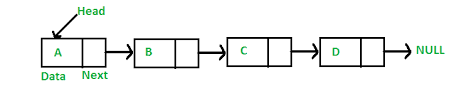
\includegraphics[width=\textwidth]{./img/ll-1.png}
      \end{figure}
    \end{column}
    \begin{column}{.5\textwidth}
      \begin{figure}
        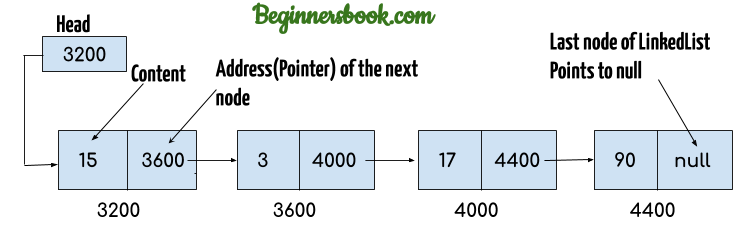
\includegraphics[width=\textwidth]{./img/ll-2.png}
      \end{figure}
    \end{column}
  \end{columns}
\end{frame}

\begin{frame}[fragile]
  \frametitle{linked list in C}
  \begin{itemize}
    \item
      linked list is implemented by
      \textbf{\color{YellowOrange} struct} and
      \textbf{\color{LimeGreen} pointer to struct}
    \item Struct has a member to save the info
    \item Struct has a pointer to point the next node
    \begin{minted}[bgcolor=Black]{c}
struct node{
  int info;
  struct node *next;
};
    \end{minted}
  \end{itemize}
\end{frame}

\begin{frame}[fragile]
  \begin{block}{}
    Please note that we <span class="hl-red">cannot</span> have structures that
    <span class="hl-green">contain themselves</span>:
  \end{block}
  \begin{minted}[bgcolor=Black]{c}
struct node{
  int info;
  struct node next;
}; // compile error
  \end{minted}
  \begin{block}{}
    <span class="hl-orange">struct node</span> conatins a pointer to its type.
  \end{block}
\end{frame}

\begin{frame}
  \frametitle{Create nodes}
  \begin{itemize}
    \item We need a function to create each node in list. The function does:
    <ol>
      \item <span class="hl-orange">Allocate</span> the memory
      \item Set the <span class="hl-green">info</span> member
      \item Set the <span class="hl-cyan">next</span> member
      \item <span class="hl-violet">Return</span> the pointer to new node
    </ol>
  \end{itemize}
\end{frame}

\begin{frame}[fragile]
  \frametitle{Create Node}
  \begin{minted}[bgcolor=Black]{c}
struct node{
  int info;
  struct node *next;
};


// Returning pointer!?!
// Is it safe?
// Why?
struct node* node_construct(int i) {
  struct node* nn = NULL;

  nn = malloc(sizeof(struct node));
  if (nn == NULL) {
   return NULL;
  }

  nn->info = i;
  nn->next = NULL;

  return nn;
}
  \end{minted}
\end{frame}

\begin{frame}
  \begin{block}{}
    We <span class="hl-orange">can return</span> the address of
    <span class="hl-green">heap-allocated</span> variables
    <span class="hl-violet">from functions</span>. Heap variables are under our
    control, so they are <span class="hl-cyan">continue existing</span> after
    the function completes.
  \end{block}
\end{frame}

\begin{frame}[fragile]
  \frametitle{Example: 3 Nodes List}
  \begin{minted}[bgcolor=Black]{c}
struct node* list = NULL;
list = node_construct(10);
list->next = node_construct(20);
list->next->next = node_construct(30);
  \end{minted}
\end{frame}

\begin{frame}
  \frametitle{Operation on linked list}
  \begin{itemize}
    \item Print the list: \texttt{\color{Orange} list\_print}
    \item
      Add new node to end of list:
      \texttt{\color{LimeGreen} list\_push\_back}

    \item
      Add new node to front of list:
      \texttt{\color{Yellow} list\_push\_front}

    \item
      Insert new node after some node:
      \texttt{\color{Cyan} list\_push\_next}

    \item
      Delete the first node in list:
      \texttt{\color{Violet} list\_pop\_front}

    \item
      Delete the end node in list:
      \texttt{\color{RubineRed} list\_pop\_back}

    \item
      Delete a node from the middle of list:
      \texttt{\color{RedOrange} list\_pop\_next}

  \end{itemize}
\end{frame}

\begin{frame}[fragile]
  \frametitle{list\_print}
  \begin{minted}[bgcolor=Black]{c}
void list_print(struct node *head){
  struct node* current;

  for(current = head; current != NULL; current = current-> next) {
    printf("%d\n", current->info)
  }
}
  \end{minted}
\end{frame}

\begin{frame}[fragile]
  \frametitle{list\_push\_back}
  \begin{minted}[bgcolor=Black]{c}
void list_push_back(struct node* head, struct node* nn){
  struct node* current;

  for(current = head; current-> next != NULL; current = current-> next);

  current->next = nn;
  nn->next = NULL;
}
  \end{minted}
\end{frame}

\begin{frame}[fragile]
  \frametitle{list\_pop\_back (if more than 1 nodes)}
  \[X \rightarrow Y \rightarrow NULL\]
  \begin{itemize}
    \item \mintinline{c}|Y = X->next|
  \end{itemize}
  \begin{enumerate}
    \item \mintinline{c}|free(Y)|
    \item \mintinline{c}|X->next = NULL|
  \end{enumerate}
\end{frame}

\begin{frame}[fragile]
  \begin{minted}[bgcolor=Black]{c}
void list_pop_back(struct node* head) {
  struct node* current = head;
  while(current->next->next != NULL) {
    current = current->next;
  }

  free(current->next);
  current->next = NULL;
}
  \end{minted}
\end{frame}

\begin{frame}[fragile]
  \frametitle{list\_push\_front 🤔}
  \begin{minted}[bgcolor=Black]{c}
void list_push_front(struct node* head, struct node* nn) {
  nn->next = list;
  head = nn;
}
  \end{minted}
\end{frame}

\begin{frame}[fragile]
  \frametitle{list\_push\_front 😱}
  \begin{minted}[bgcolor=Black]{c}
void list_push_front(struct node** phead, struct node* nn) {
  nn->next = *phead;
  *phead = nn;
}
  \end{minted}
\end{frame}

\begin{frame}[fragile]
  \frametitle{list\_pop\_next}
  \[X \rightarrow Y \rightarrow Z\]
  \begin{itemize}
    \item \mintinline{c}|Y = X->next|
    \item \mintinline{c}|Z = Y->next|
    \item \mintinline{c}|Z = X->next->next|
  \end{itemize}
  \begin{enumerate}
    \item \mintinline{c}|X->next = Z|
    \item \mintinline{c}|free(Y)|
  \end{enumerate}
\end{frame}
\begin{frame}[fragile]
  \frametitle{list\_pop\_next}
  \begin{minted}[bgcolor=Black]{c}
void list_pop_by_info(struct node* head, int v) {
  // find a node before the node that contains v
  struct node* current = head;
  for (current = list; current->next != NULL && current->next->info != v; current = current->next);

  // there is no node that conaints v
  if (current->next == NULL) {
    return;
  }

  list_pop_next(current);
}
  \end{minted}
\end{frame}
\begin{frame}[fragile]
  \frametitle{list\_pop\_next}
  \begin{minted}[bgcolor=Black]{c}
void list_pop_next(struct node* adjacent_to_delete_node) {
  struct node* to_delete = adjacent_to_delete_node->next;
  adjacent_to_delete_node->next = to_delete->next;
  free(to_delete);
}
  \end{minted}
\end{frame}

\begin{frame}
  \frametitle{Common Bugs}
  \begin{itemize}
    \item
      The last <span class="hl-orange">NULL</span> in Liked-list is very
      important

    \begin{itemize}
      \item Always keep it
    \end{itemize}
    \item Operation of linked-list has many exceptions
    \begin{itemize}
      \item When list is empty
      \item When we want to add to the first of list
      \item \ldots
    \end{itemize}
  \end{itemize}
\end{frame}

\section{Enum Definition}

\begin{frame}
  \frametitle{Introduction}
  \begin{itemize}
    \item Some data are naturally ordered
    \begin{itemize}
      \item Days of week
      \item Months of year
    \end{itemize}
    \item We want to use the order, e.g.
    \begin{itemize}
      \item The number of visitors per day
      \item The salary per month
    \end{itemize}
    \item We need an array
    \begin{itemize}
      \item
        visitors[<span class="hl-green">0</span>] \textrightarrow The number of visitors
        in <span class="hl-orange">Saturday</span>

      \item
        visitors[<span class="hl-green">1</span>] \textrightarrow The number of visitors
        in <span class="hl-orange">Sunday</span>

    \end{itemize}
  \end{itemize}
\end{frame}

\begin{frame}[fragile]
  \frametitle{Introduction}
  \begin{itemize}
    \item
      \textbf{\color{YellowOrange} Enumeration} is a mechanism to assign a name
      for each number

    \item We can use numbers instead of numbers
    \begin{itemize}
      \item More readable core
    \end{itemize}
    \item E.g.
    \begin{minted}[bgcolor=Black]{c}
visitors[saturday], visitors[friday]
salary[april], salary[june]
    \end{minted}
  \end{itemize}
\end{frame}

\begin{frame}[fragile]
  \frametitle{enum}
  \begin{itemize}
    \item
      \textit{\color{LimeGreen} enum} is used to define a set of names and
      their corresponding numbers

    \begin{minted}[bgcolor=Black]{c}
enum tag {name_1, name_2, ..., name_N};
    \end{minted}
    \item \textsc{\color{Yellow} tag} is the enumeration type
    \begin{itemize}
      \item We use it to define variables
    \end{itemize}
    \item
      $name_1$ is $0$
    \item
      $name_2$ is $1$
    \item
      $name_{i}$ is $name_{i-1} + 1$

  \end{itemize}
\end{frame}

\begin{frame}[fragile]
  \frametitle{enum}
  \begin{minted}[bgcolor=Black]{c}
enum week {sat, sun, mon, tue, wed, thu, fri};
  \end{minted}
  sat = 0, sun = 1, mon = 2, \ldots, fri = 6

  \begin{minted}[bgcolor=Black]{c}
enum year {feb, jan, mar, apr, may, jun, jul, aug, sep, oct, nov, des};
  \end{minted}
  feb = 0, jan = 1, \ldots, nov = 10, des = 11
\end{frame}

\begin{frame}[fragile]
  \frametitle{enum}
  <p>We can assign the numbers</p>
  \begin{minted}[bgcolor=Black]{c}
enum week {sat = 1, sun, mon, tue, wed, thu, fri};
  \end{minted}
  <p>sat = 1, sun = 2, mon = 3, …, fri = 7</p>
  \begin{minted}[bgcolor=Black]{c}
enum condition {False = 0, True, No = 0, Yes, Ghalat = 0, Dorost};
  \end{minted}
  \begin{minted}[bgcolor=Black]{output}
    False = No = Ghalat = 0
    True = Yes = Dorost = 1
  \end{minted}
\end{frame}

\begin{frame}[fragile]
  \frametitle{enum}
  \begin{itemize}
    \item After definition of an enumeration
    \item We can use the tag to declare variables
    \item We can use the names to assign values to the variables
  \end{itemize}
  \begin{minted}[bgcolor=Black]{c}
enum week { sat, sun, mon, tue, wed, thu, fri };
enum week day = sat;
for(day = sat; day <= fri; day++)
  \end{minted}
\end{frame}

\begin{frame}[fragile]
  \frametitle{Example: Read the number of visitors}
  \begin{minted}[bgcolor=Black]{c}
enum week {sat, sun, mon, tue, wed, thu, fri};
int visitors[7];
enum week day;
for(day = sat; day <= fri; day++)
  scanf("%d", &visitors[day]);
  \end{minted}
\end{frame}

\begin{frame}[fragile]
  \frametitle{Caution}
  \begin{itemize}
    \item
      C compiler \textsc{\color{RubineRed} does not} check the value is
      assigned to the enum variables

    \begin{minted}[bgcolor=Black]{c}
enum test1 {t1, t2, t3};
enum test2 {t4, t5, t6};
enum test1 t1v = t1;
enum test2 t2v = t4;
if(t1v == t2v) // true
t1v = t5;
t2v = 100;
    \end{minted}
  \end{itemize}
\end{frame}

\section{Union Definition}

\begin{frame}
  \frametitle{Introduction}
  \begin{itemize}
    \item
      Like Structures,
      \textsc{\color{Orange} union is a user defined data type}.
    \item In union, all members share the same memory location.
  \end{itemize}
\end{frame}

\begin{frame}
  \frametitle{Introduction}
  \begin{figure}
  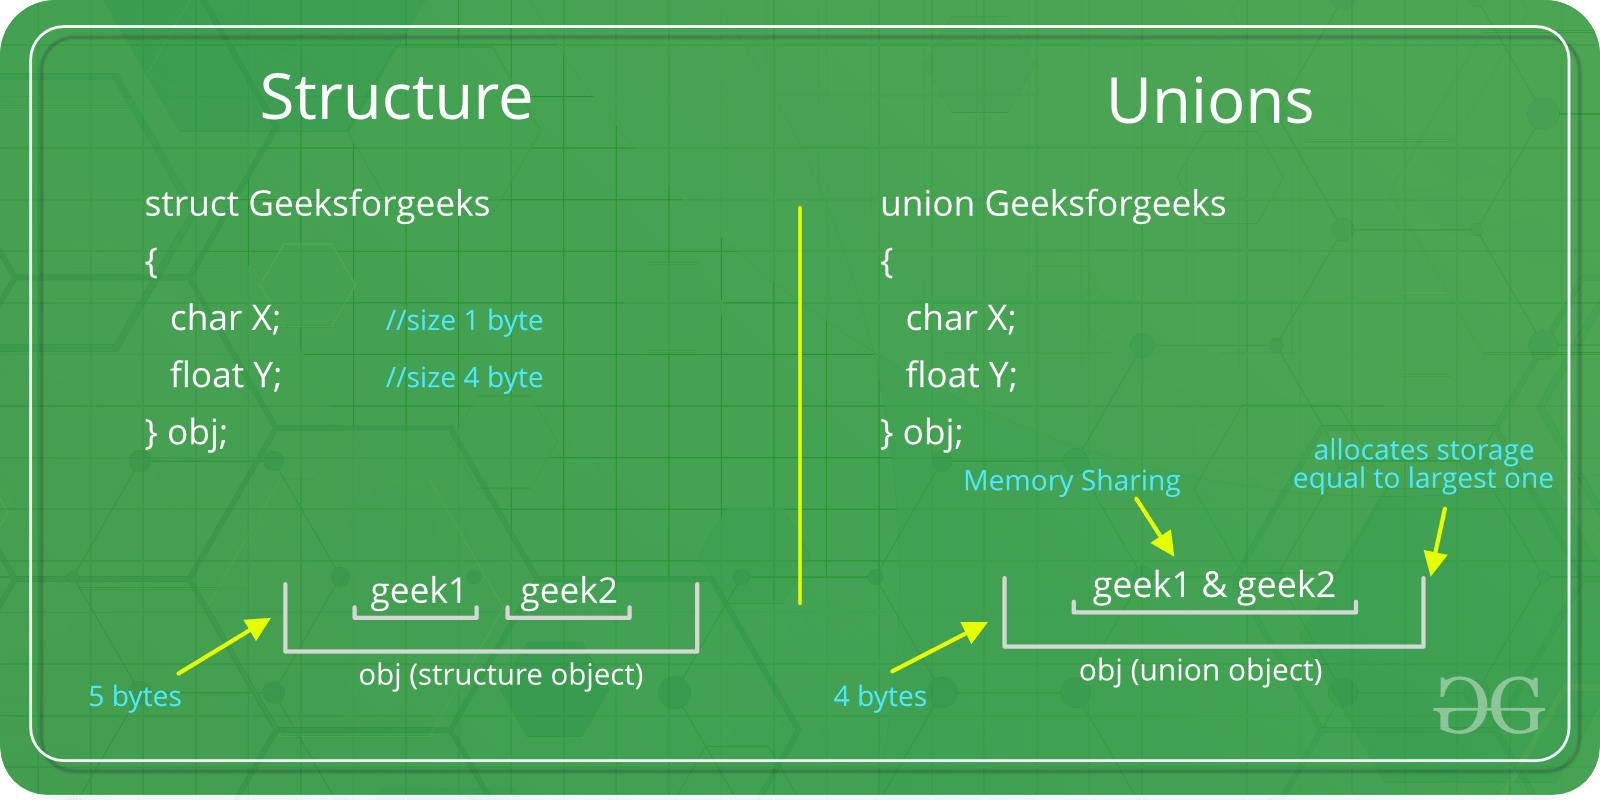
\includegraphics[width=\textwidth]{./img/union.png}
  \end{figure}
\end{frame}

\begin{frame}[fragile]
  \scriptsize
  \begin{minted}[bgcolor=Black]{c}
#include <stdio.h>

// Declaration of union is same as structures
union test {
    int x, y;
};

int main()
{
    // A union variable t
    union test t;

    t.x = 2; // t.y also gets value 2
    printf("After making x = 2:\n x = %d, y = %d\n\n",
           t.x, t.y);

    t.y = 10; // t.x is also updated to 10
    printf("After making y = 10:\n x = %d, y = %d\n\n",
           t.x, t.y);
    return 0;
}
  \end{minted}
  \begin{minted}[bgcolor=Black]{output}
After making x = 2:
 x = 2, y = 2

After making y = 10:
 x = 10, y = 10
  \end{minted}
\end{frame}

\begin{frame}[fragile]
  \scriptsize
  \begin{minted}[bgcolor=Black]{c}
#include <stdio.h>

union test1 {
    int x;
    int y;
} Test1;

union test2 {
    int x;
    char y;
} Test2;

union test3 {
    int arr[10];
    char y;
} Test3;

int main()
{
    printf("sizeof(test1) = %lu, sizeof(test2) = %lu, "
           "sizeof(test3) = %lu",
           sizeof(Test1),
           sizeof(Test2), sizeof(Test3));
    return 0;
}
  \end{minted}

  \begin{minted}[bgcolor=Black]{output}
sizeof(test1) = 4, sizeof(test2) = 4, sizeof(test3) = 40
  \end{minted}
\end{frame}

\begin{frame}
  \frametitle{Legends}
  \begin{figure}
    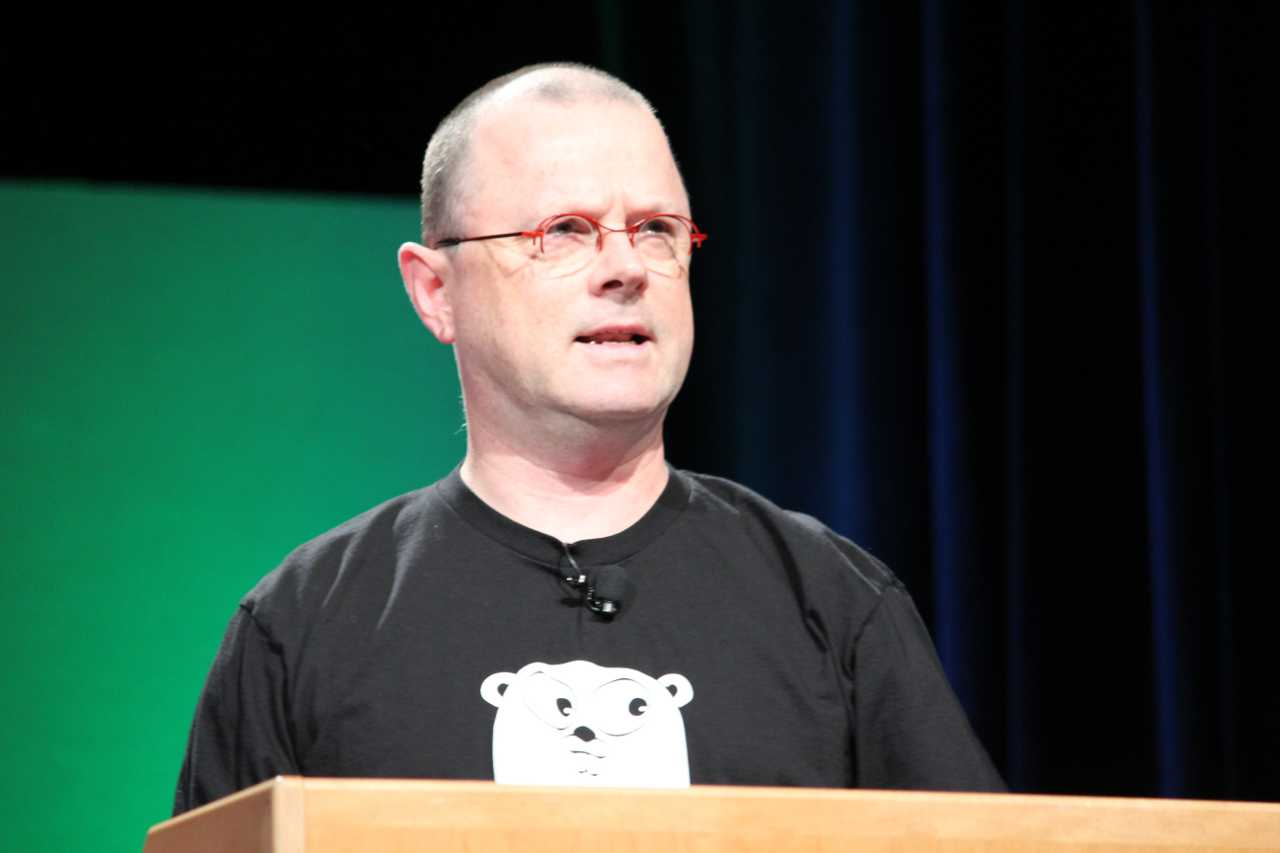
\includegraphics[height=.75\textheight]{./img/rob.jpg}
  \end{figure}
  \pause%
  \centering
  \color{Violet} Rob Pike
\end{frame}

\begin{frame}
  \frametitle{Legends}
  \begin{itemize}
    \item Canadian programmer and author
    \item
      He is best known for his work on the Go programming language and at Bell
      Labs
  \end{itemize}
\end{frame}

\end{document}
